\section{Geo-zones}
Geo-zones represent a simple geographical polygons that can ``guard'' machine movements and store 
intersection events to refer them later.

\begin{figure}[!htp]
\centering
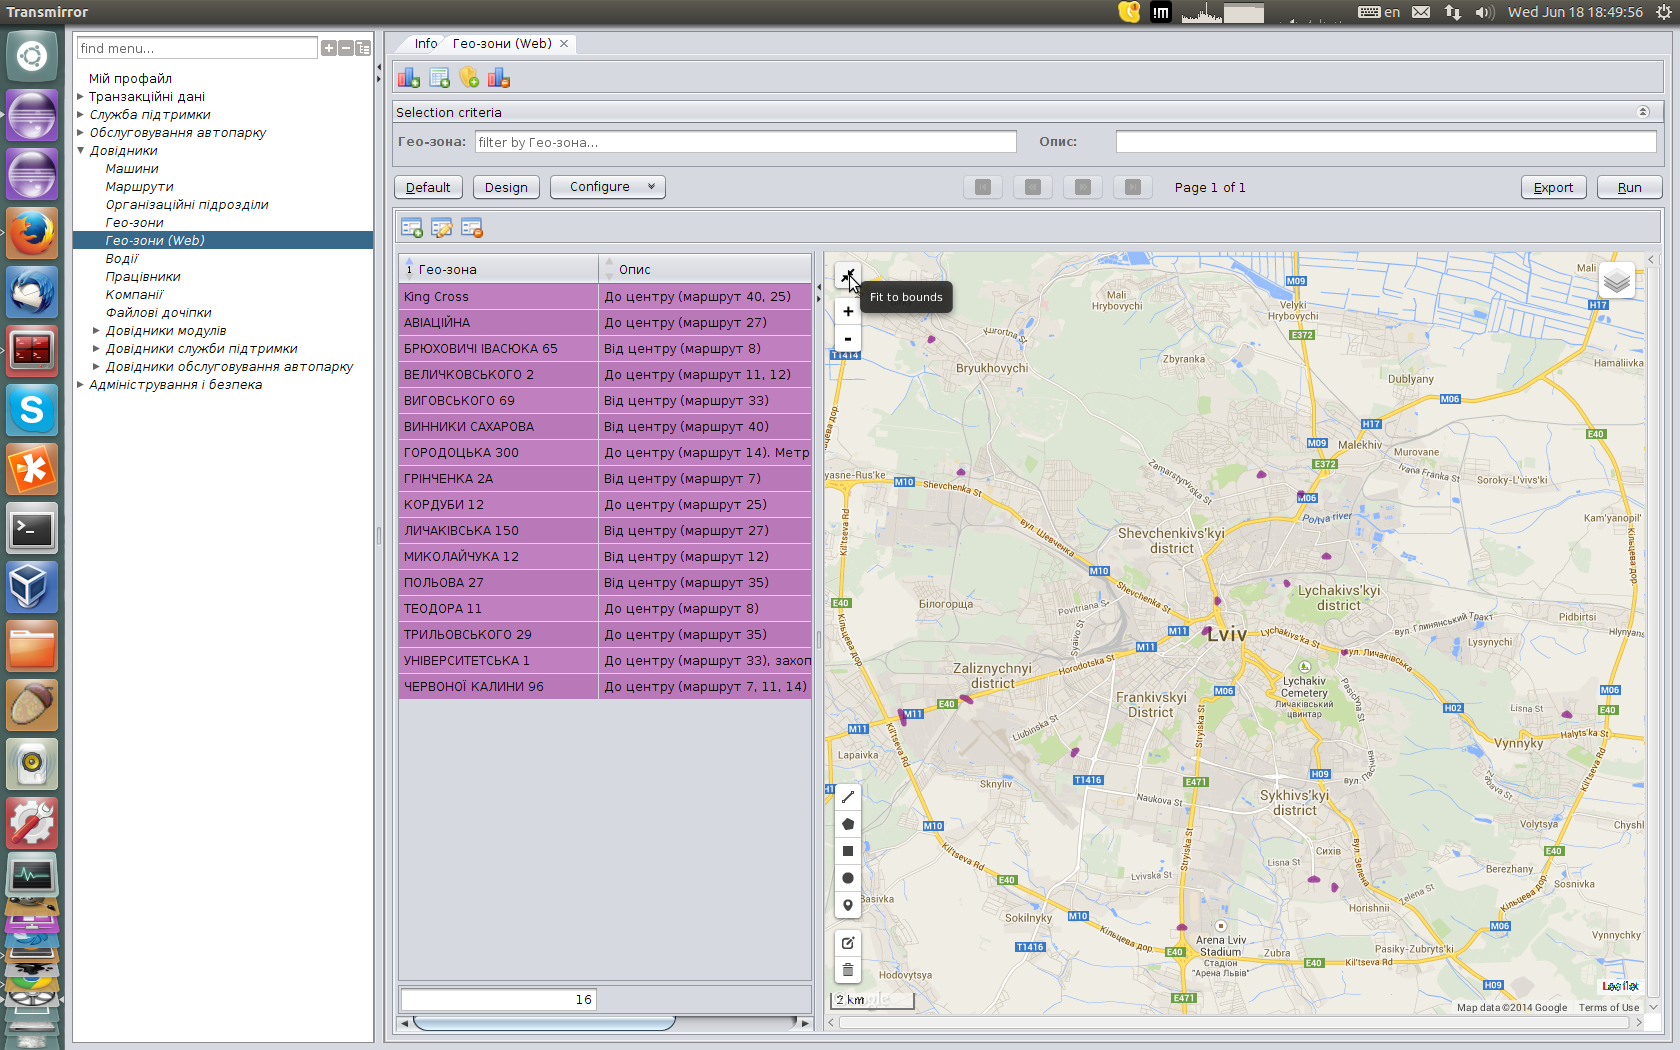
\includegraphics[width=16cm]{chapters/01-geozones/images/01-all-geo-zones-using-fit-to-bounds-button.png}
\caption{all-geo-zones-using-fit-to-bounds-button}\label{fig:01}
\end{figure}

\begin{figure}[!htp]
\centering
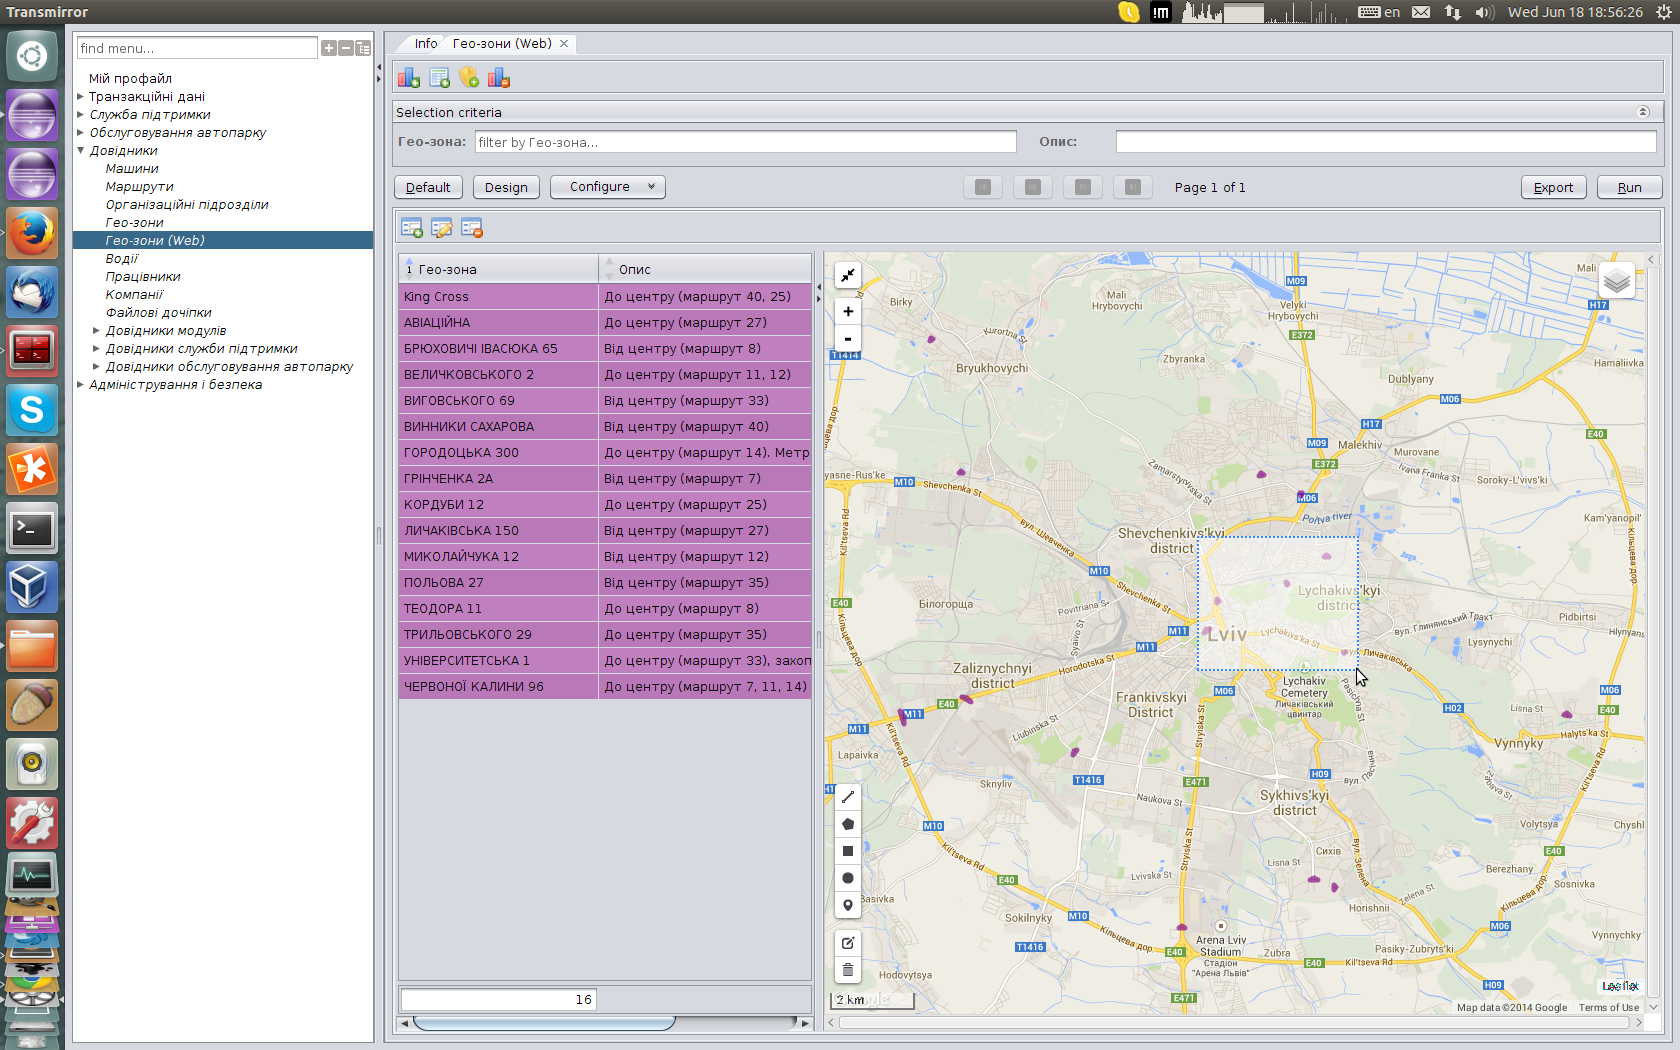
\includegraphics[width=16cm]{chapters/01-geozones/images/02-part-of-geo-zones-using-shift+selection-zoom.png}
\caption{part-of-geo-zones-using-shift+selection-zoom}\label{fig:02}
\end{figure}

\begin{figure}[!htp]
\centering
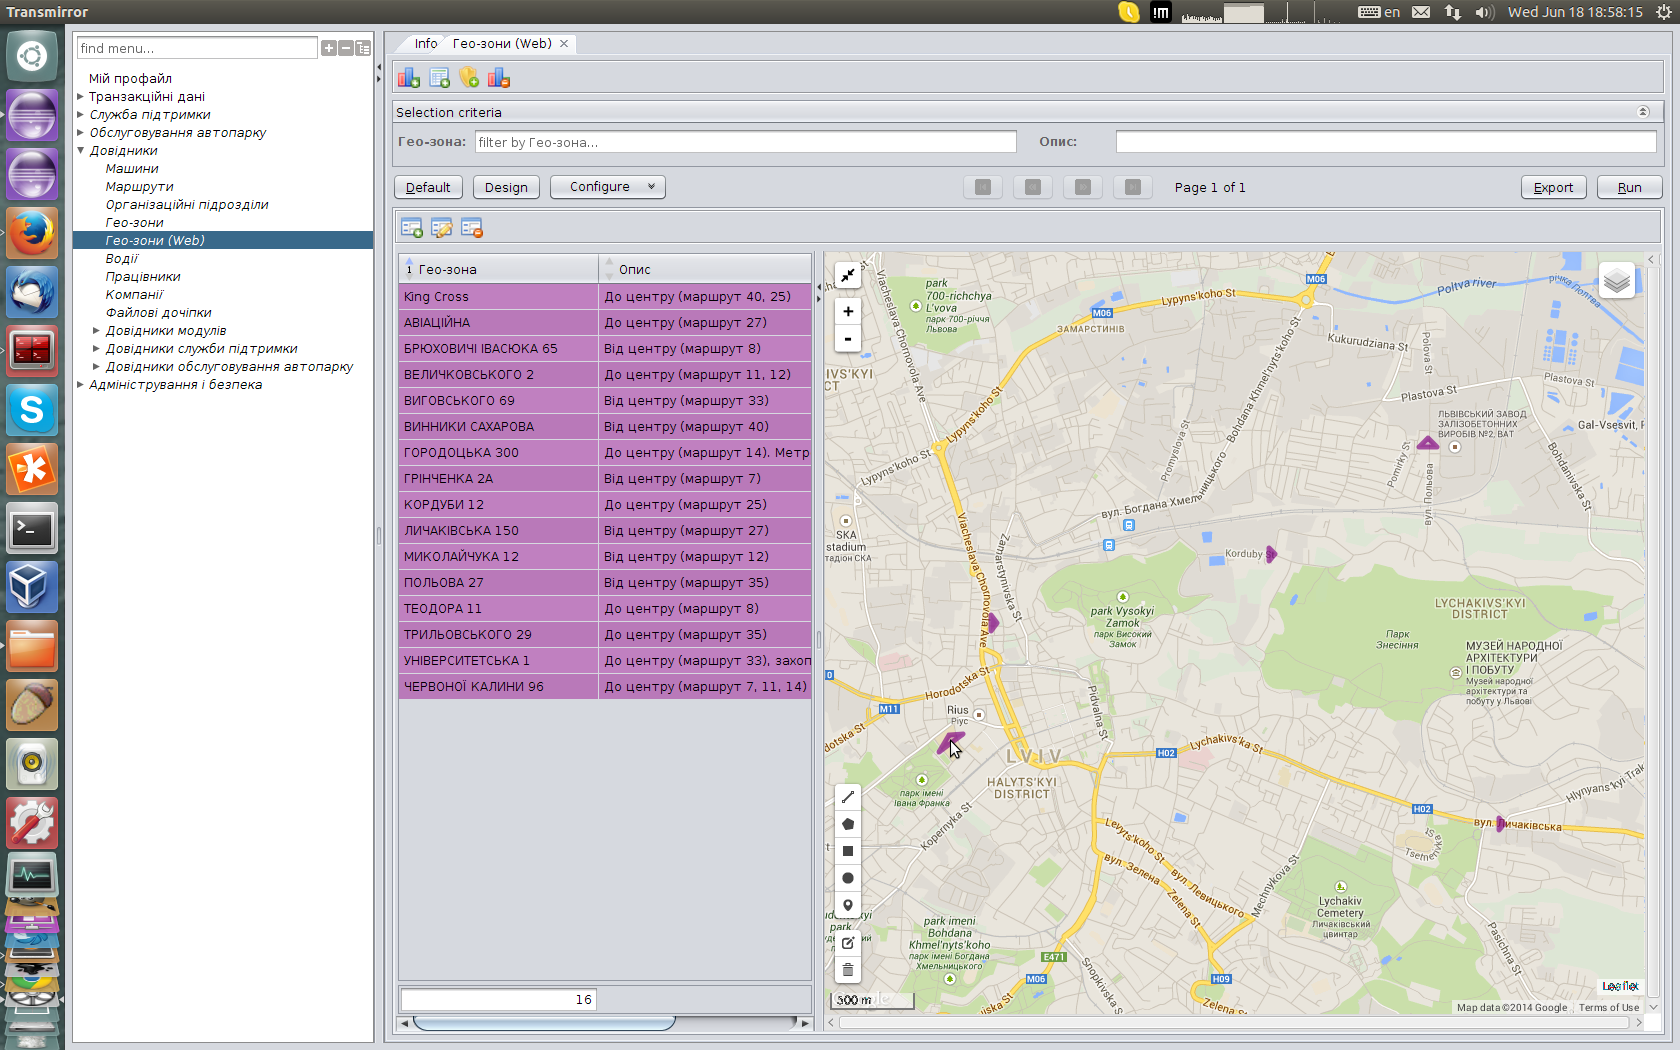
\includegraphics[width=16cm]{chapters/01-geozones/images/03-part-of-geo-zones-with-particular-item-selection-by-clicking.png}
\caption{part-of-geo-zones-with-particular-item-selection-by-clicking}\label{fig:03}
\end{figure}

\begin{figure}[!htp]
\centering
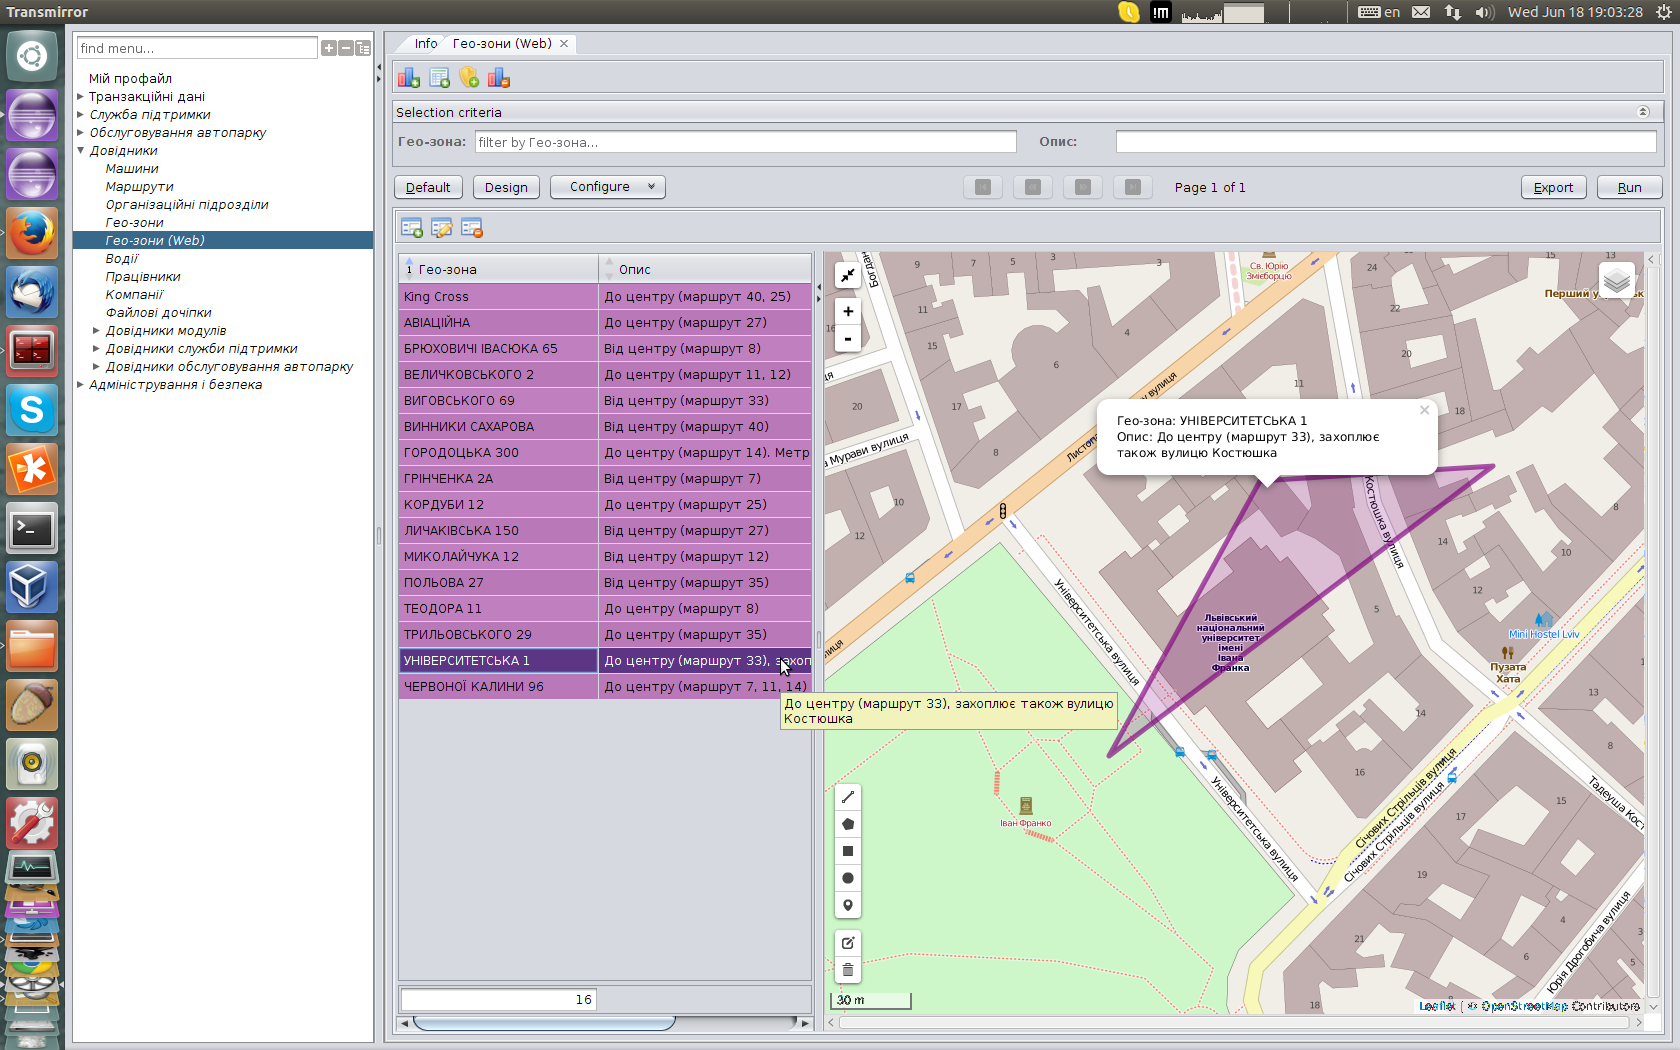
\includegraphics[width=16cm]{chapters/01-geozones/images/04-selected-geo-zone-and-synchronised-with-grid.png}
\caption{selected-geo-zone-and-synchronised-with-grid}\label{fig:04}
\end{figure}

\begin{figure}[!htp]
\centering
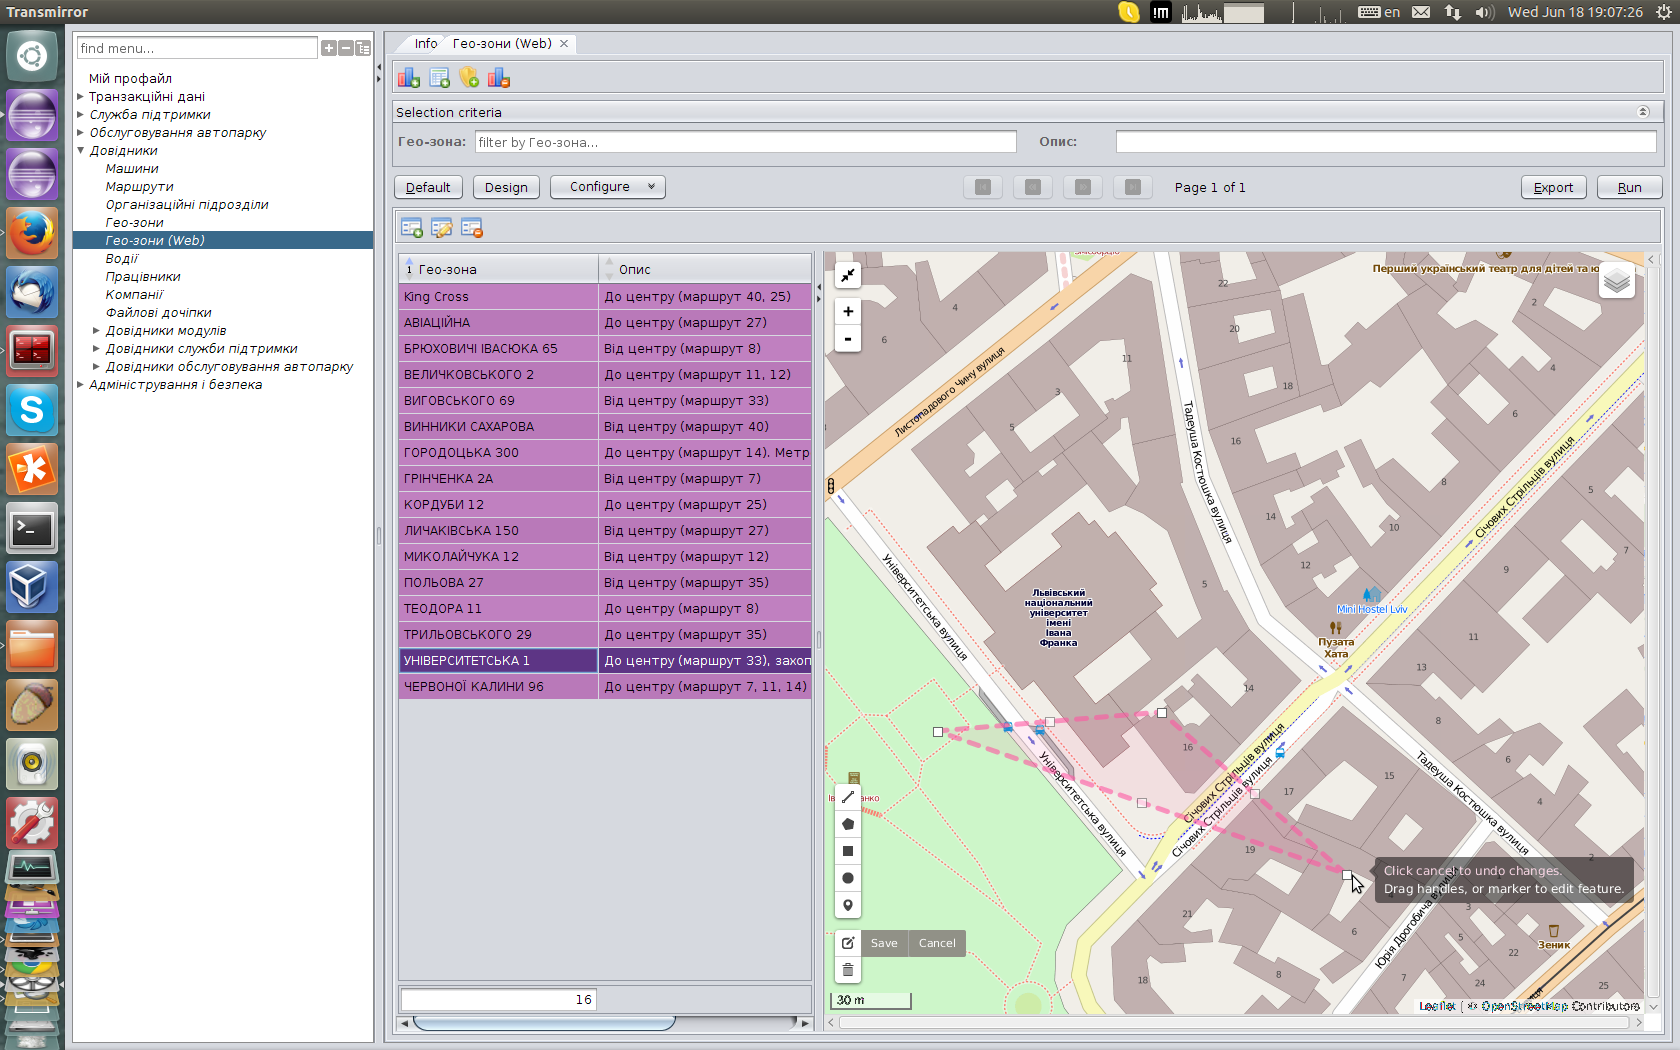
\includegraphics[width=16cm]{chapters/01-geozones/images/05-editing-geo-zone-using-graphical-interface.png}
\caption{editing-geo-zone-using-graphical-interface}\label{fig:05}
\end{figure}

\begin{figure}[!htp]
\centering
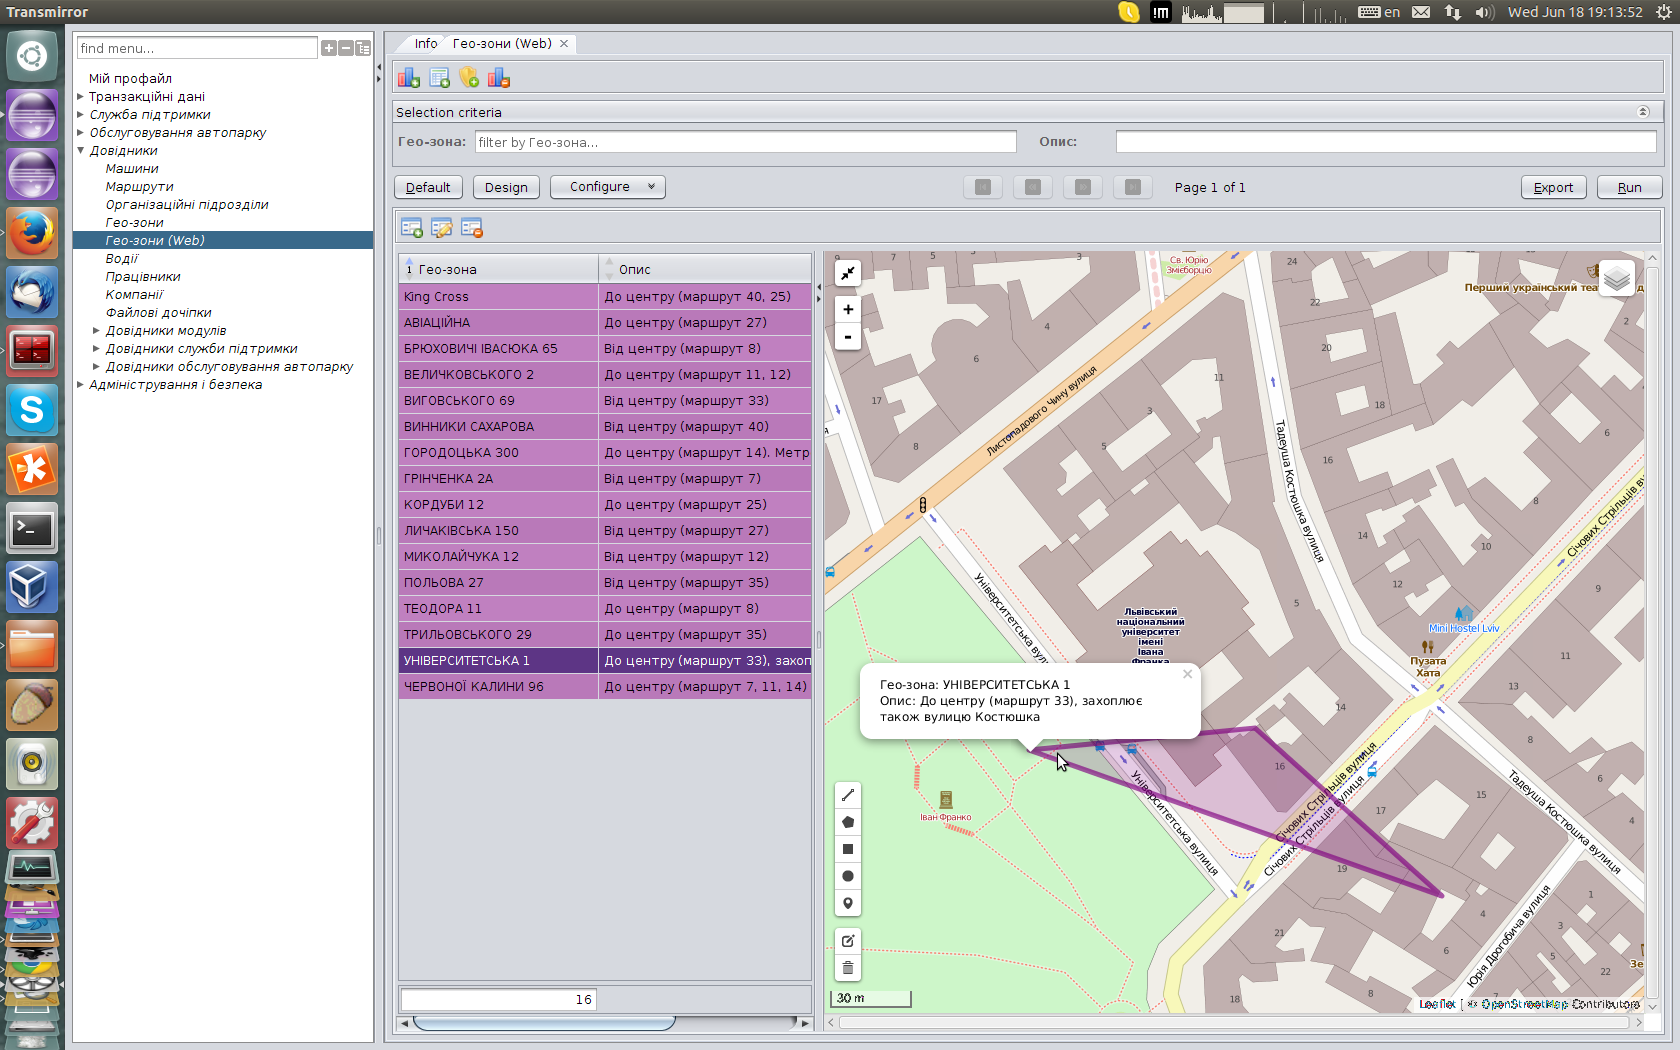
\includegraphics[width=16cm]{chapters/01-geozones/images/06-edited-geo-zone.png}
\caption{edited-geo-zone}\label{fig:06}
\end{figure}

\begin{figure}[!htp]
\centering
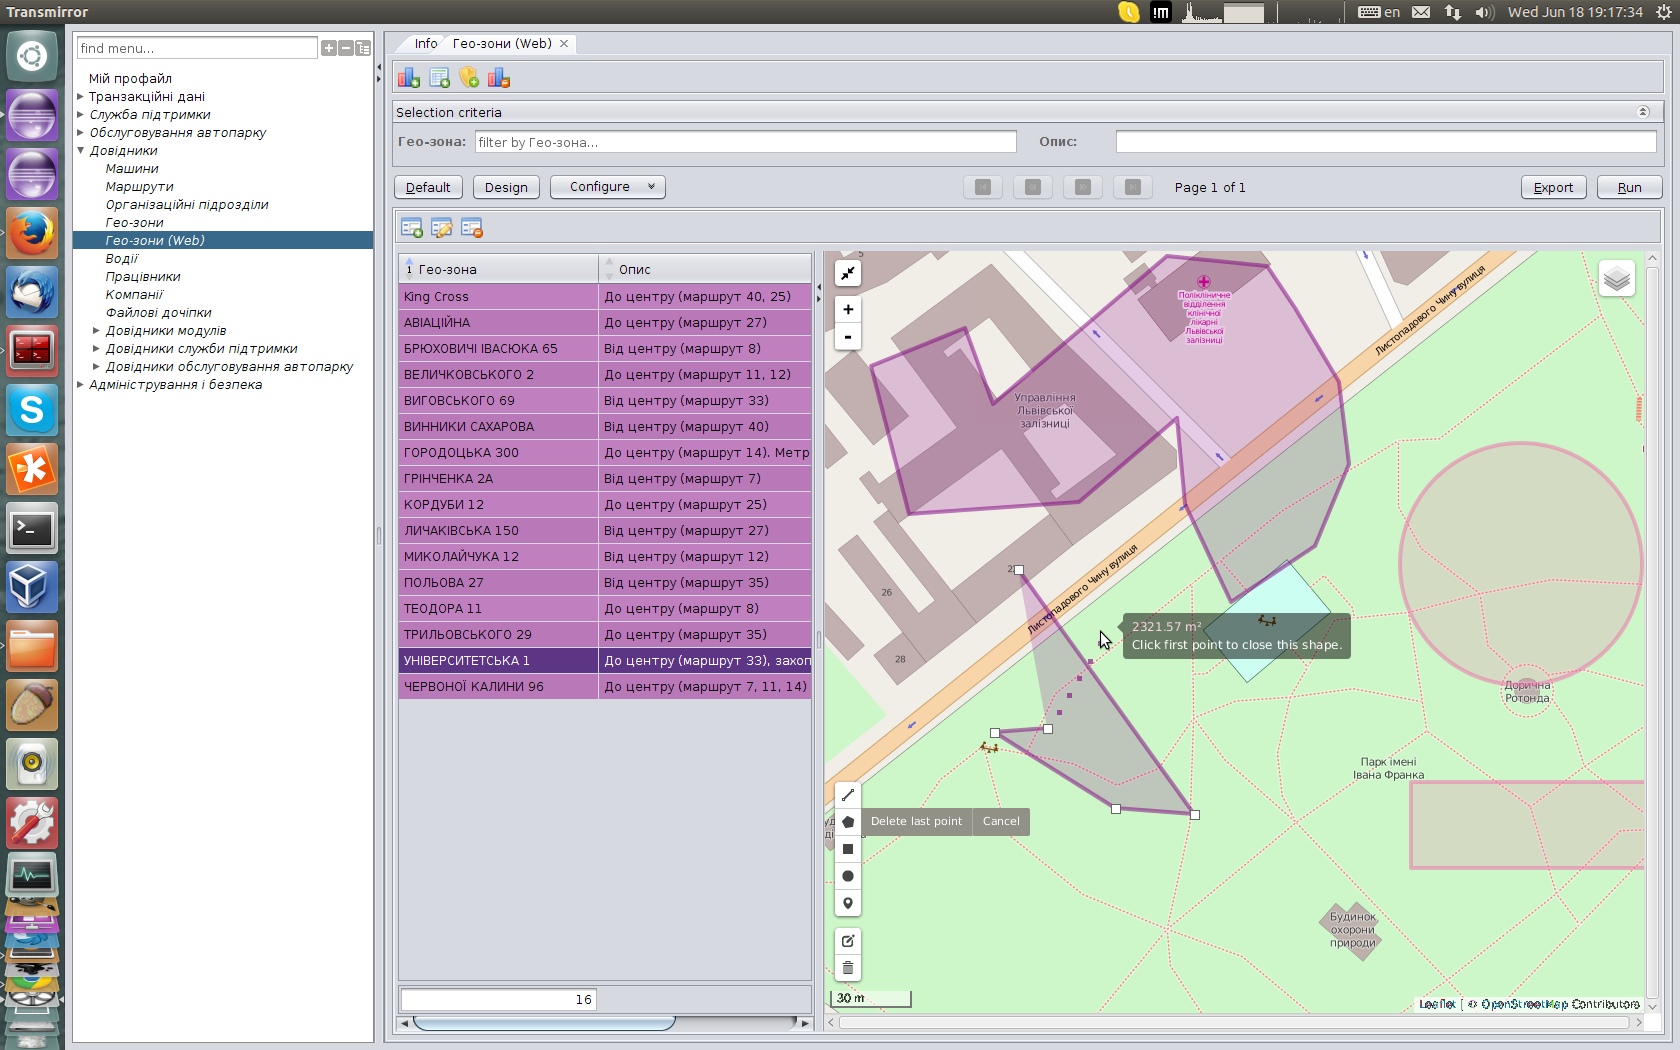
\includegraphics[width=16cm]{chapters/01-geozones/images/07-creating-new-complex-geo-zones.png}
\caption{creating-new-complex-geo-zones}\label{fig:07}
\end{figure}

\begin{figure}[!htp]
\centering
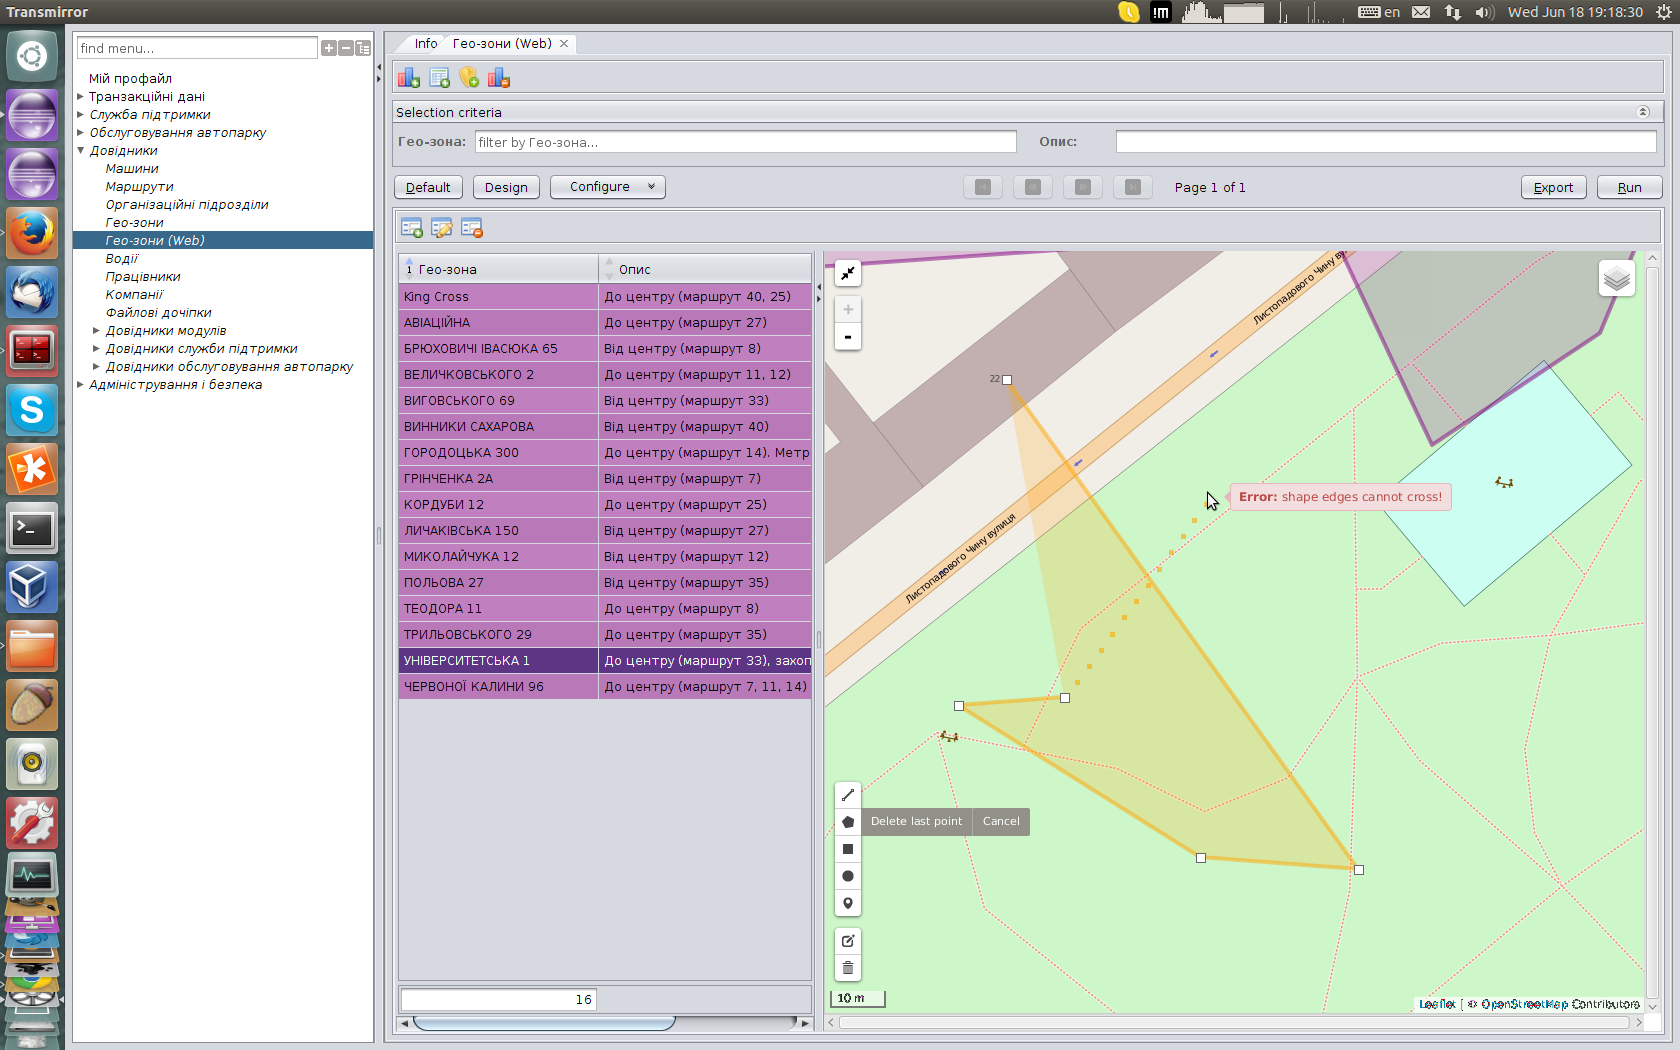
\includegraphics[width=16cm]{chapters/01-geozones/images/08-validation-for-complex-polygonial-geozone.png}
\caption{validation-for-complex-polygonial-geozone}\label{fig:08}
\end{figure}

\begin{figure}[!htp]
\centering
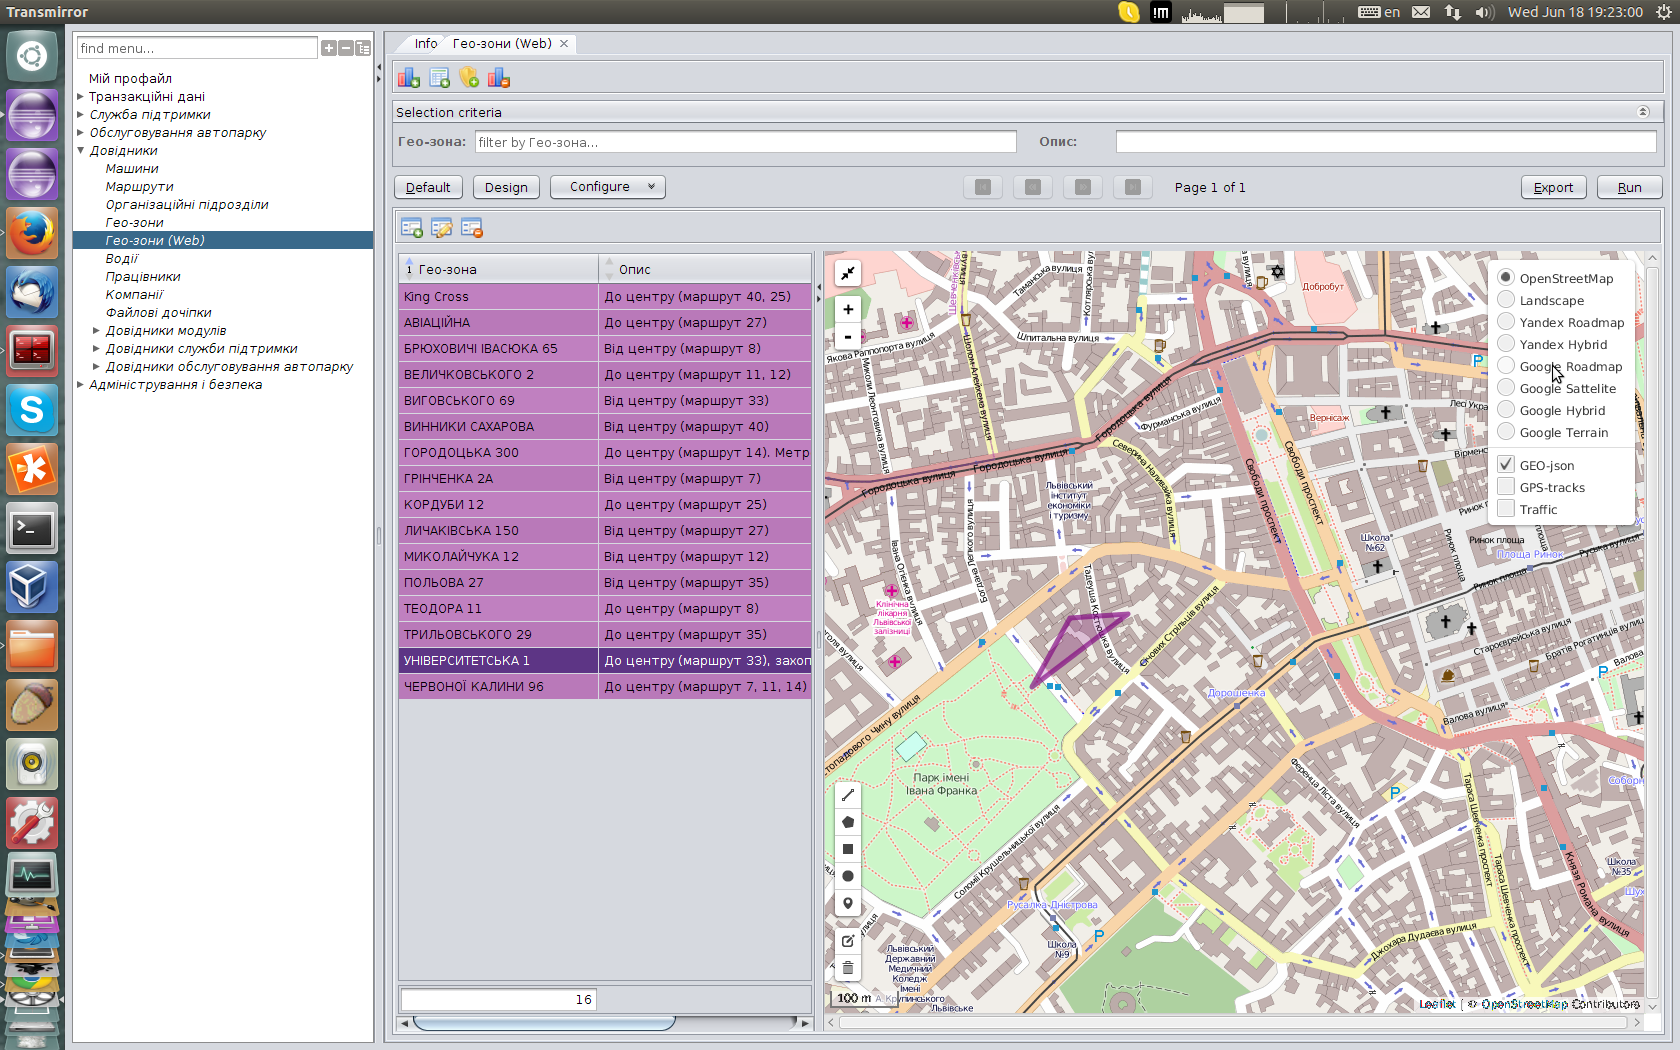
\includegraphics[width=16cm]{chapters/01-geozones/images/09-changing-map-tiling-service.png}
\caption{09-changing-map-tiling-service}\label{fig:09}
\end{figure}

\begin{figure}[!htp]
\centering
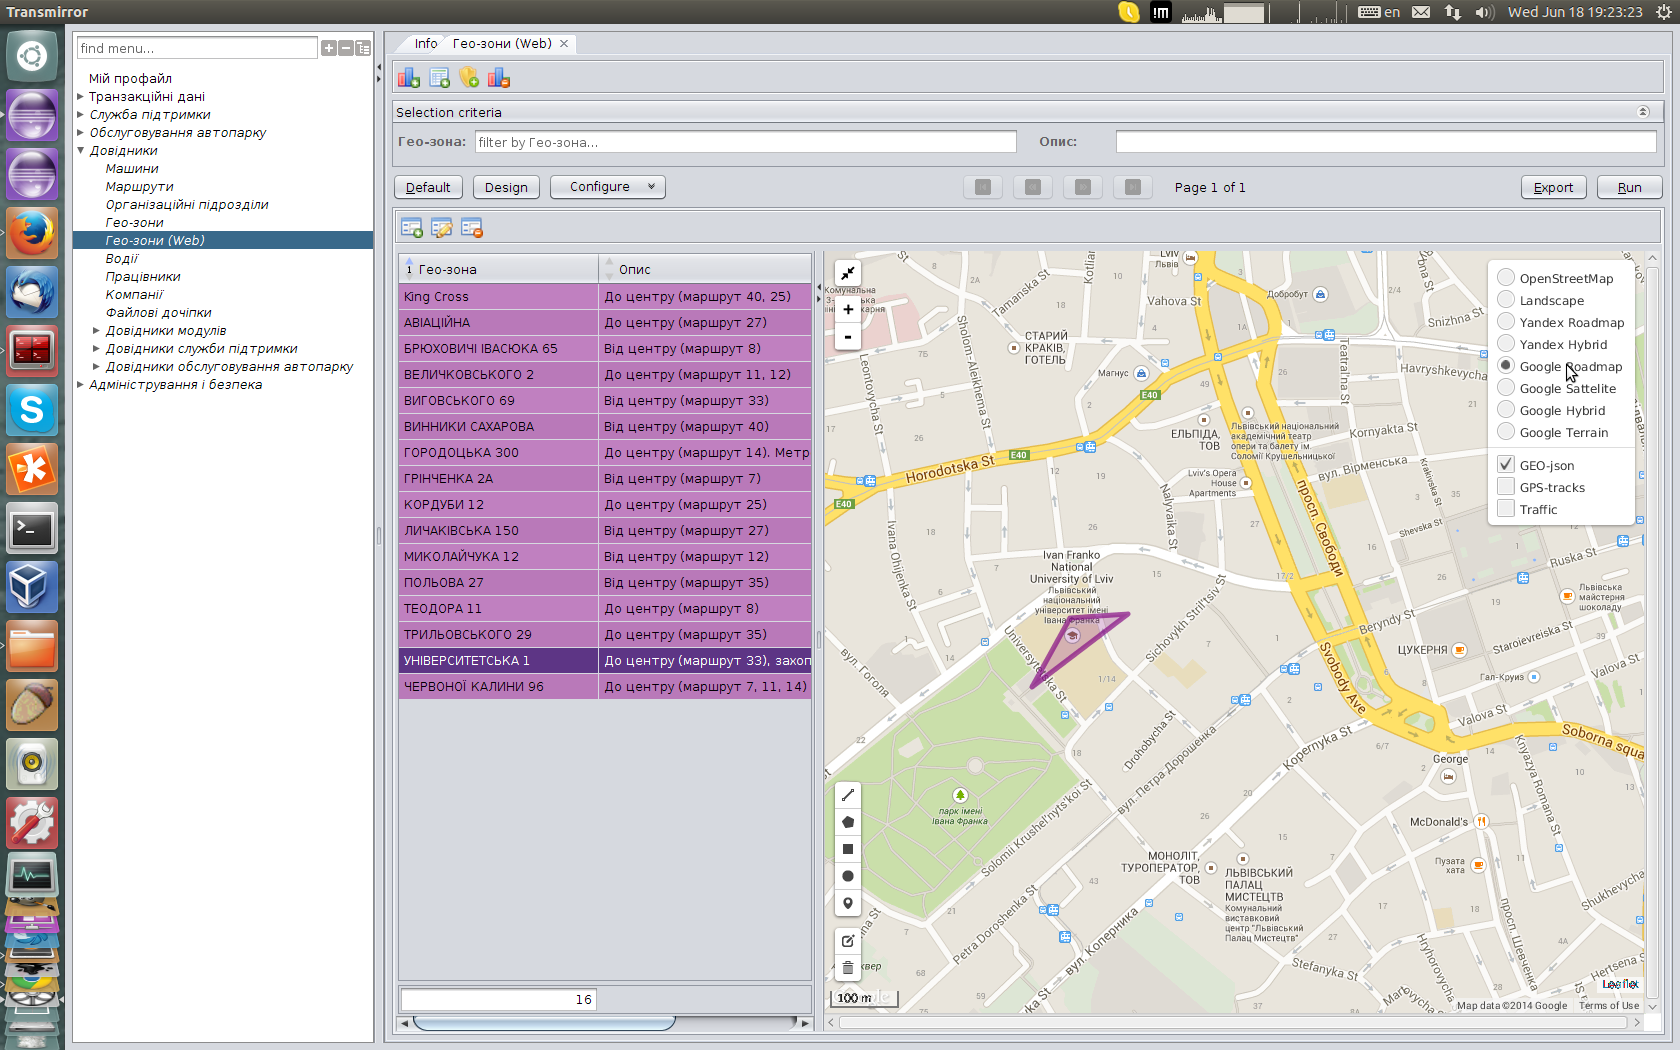
\includegraphics[width=16cm]{chapters/01-geozones/images/10-changed-map-tiling-service.png}
\caption{changed-map-tiling-service}\label{fig:10}
\end{figure}